%--------Marco Teórico
%--------Daniel Ochoa John
%--------20/07/2014
\renewcommand{\thefigure}{\thechapter-\arabic{figure}}

\chapter{Marco Teórico}

\label{cap:marcoteorico}

En este capítulo se exponen los fundamentos teóricos del trabajo de tesis. Primero, se define el concepto de red social y sus formas de representación. Luego, se explora el concepto de análisis de redes sociales orientado principalmente a la detección de comunidades. Posteriormente, se define el concepto de sistema de recomendación, analizando aquellos conceptos que son considerados en este trabajo de tesis. Finalmente, se describe la lógica de la 3-Ontology, junto con un repaso de lo realizado anteriormente en relación a este concepto.

\section{Redes Sociales}

Las relaciones interpersonales son básicas para todo ser humano y están presentes en nuestra vida cotidiana, interactuamos con personas a cada momento y en cada lugar. Sociológicamente hablando, es posible definir el concepto de relación interpersonal como el total de interacciones que generan las personas en un contexto determinado (Dalton, 2007).

Estas interacciones pueden presentarse en distintos ámbitos, como por ejemplo, personales o laborales. Si se abstrae este concepto de relación interpersonal, es posible compararlo al contexto actual en lo que se conoce como una red social. Una red social es una estructura compuesta por nodos (individuos u organizaciones) y aristas, que conectan a los nodos formando una relación. Dichas relaciones pueden deberse a distintos tipos de interacciones como amistad, interés, entre otras.

Existen métodos para la representación de redes sociales, no obstante típicamente son utilizados dos. Uno es gráficamente mediante el renderizado de un grafo, otro es a través de una matriz de adyacencia (Wasserman & Faust, 1994). Las aristas en las redes sociales pueden contener distintos atributos, como peso, signo y dirección. Cuando las aristas contienen peso, es que a ellas se ha asociado un valor numérico que mide la relación en cierto aspecto (calidad, cercanía, similitud, entre otros), el signo puede determinar si la relación entre dos nodos es positiva o negativa, finalmente la dirección indica el sentido en el que la relación está definida.

\section{An\'alisis de Redes Sociales}

Las redes sociales en un contexto de \textit{social media} son generalmente muy grandes, con millones de usuarios y conexiones entre ellos. Haciendo uso de las capacidades únicas de masividad que provee la \textit{social media}, estas redes están presentando desafíos con respecto a su análisis (Tang & Liu, 2010):

\begin{enumerate}[I]
	\item \textbf{Escalabilidad:} Las redes sociales pueden crecer a tamaños astronómicos, conteniendo cientos de miles de conexiones. En \textit{Facebook}, por ejemplo, es tan evidente como que la comunidad de fans del fútbol tiene un orden de magnitud de 500 millones de usuarios (Smith, 2014). El análisis de redes sociales clásico tradicionalmente maneja un orden de magnitud de cientos o menos.
	\item \textbf{Heterogeneidad:} Entre dos usuarios puede existir múltiples tipos de relaciones. En la red social Google+, se aborda este concepto a través del uso de círculos para denotar el contexto de relación entre un usuario y sus contactos. Más aún, puede existir una variedad de interacciones entre un mismo conjunto de usuarios, como por ejemplo un mensaje privado, un \textit{like}, un etiquetado en una fotografía en común. Este contenido en su conjunto es relevante para, por ejemplo, recomendar un contenido.
	\item \textbf{Evolución:} Una de las características fundamentales de \textit{social media} es su orden temporal. Por ejemplo, en \textit{Twitter}, que es una red de microblogging, el contenido relevante y de interés para la mayor parte de los usuarios (a.k.a \textit{trending topics}) cambia rápida y constantemente en cortos períodos de tiempo (Kerr, 2012). Nuevos usuarios aparecen, usuarios “veteranos” dejan de participar, nuevas conexiones se generan, en resumen todo \textit{data\textit{set}} que pertenezca a \textit{social media} es dinámico, y se debe identificar constantemente aquellos focos relevantes para el análisis, como por ejemplo nuevas comunidades emergentes.
	\item \textbf{Inteligencia Colectiva:} En \textit{social media}, las personas tienden a compartir sus conexiones y parecer respecto a distintos objetos de interés. El conocimiento generado por las masas a través de \textit{tags}, comentarios, reviews y ratings son antecedentes recabados por muchos portales Web como \textit{Amazon} o \textit{Spotify}. Conceptos como la confiabilidad y reputación de los usuarios toman relevancia y trascendencia (Victor, De Cock, & Cornelis, 2011) con el objetivo de recomendar a otros individuos conceptos (items en general) que sean de su interés.
	\item \textbf{Evaluación:} Este es un desafío ocasionado íntegramente por las barreras existentes en la obtención de información para entrenar modelos y algoritmos de análisis. Muchos sitios de \textit{social media} implementan políticas de privacidad que limitan la información a la que un agente externo puede acceder. Como experimentar con un escenario real es poco probable, es necesario aproximarse a él (Leskovec & Faloutsos, 2006; Hübler, Kriegel, Borgwardt, & Ghahramani, 2008), o bien simular condiciones similares (Chakrabarti & Faloutsos, 2006; Maiya & Berger-Wolf, 2010).
\end{enumerate}

\section{Detecci\'on de Comunidades}

En relación con la inteligencia colectiva y la evolución de las interacciones de un conjunto de usuarios en un contexto de redes sociales, las comunidades permiten caracterizar a aquellos usuarios similares. La detección de comunidades es una de las tareas fundamentales en el análisis de redes sociales, ya que permiten describir fenómenos sociales analizando el comportamiento colectivo (Hechter, 1988).

Una comunidad, en el contexto de una red social, es aquella en la que un conjunto de nodos que interactúan entre ellos más que con los que están fuera del grupo. La detección de comunidades puede ser aplicada en distintos contextos del “mundo real”, como por ejemplo, en una aplicación de contenido musical, agrupar usuarios con intereses similares y en base a esto recomienda música similar a otros usuarios. En otros casos, las comunidades pueden ser utilizadas para comprimir redes sociales muy grandes o proveer un mecanismo de exploración y navegación para grafos sociales. Es posible clasificar las diferentes líneas de investigación con respecto de la detección de comunidades (Tang & Liu, 2010).

La primera surge por la carencia de los métodos clásicos de detección utilizados en las ciencias sociales, que son incapaces de manejar el volumen de datos de las redes sociales en el contexto de \textit{social media}, y se enfoca en escalar los métodos de  detección de comunidades para que puedan manejar redes de gran tamaño (Andersen, 2007; Dourisboure, Geraci, & Pellegrini, 2007; Gibson, Kumar, & Tomkins, 2005).

La segunda línea nace para abordar el desafío de heterogeneidad, y tiene que ver con la detección de comunidades en redes con entidades e interacciones de distinta naturaleza (Java, Joshi, & Finin, 2008; Tang, Liu, Zhang, & Nazeri, 2008; Tang, Wang, & Liu, 2009), como \textit{Facebook} o \textit{YouTube}.

La tercera línea de investigación nace para abordar el desafío de evolución y tiene que ver con los cambios en el tiempo que tienen todas las redes sociales en un contexto de \textit{social media} (Asur, Parthasarathy, & Ucar, 2009; Backstrom, Dwork, & Kleinberg, 2007; Palla, Barabási, & Vicsek, 2007; Tang, Liu, & Zhang, 2012). Por ejemplo, el número de usuarios activos en \textit{Facebook} ha crecido de 1 millón de usuarios activos en 2004 a 1.11 billones de usuarios en 2013 (AP, 2013), lógicamente la cantidad y estructura de las comunidades ha cambiado debido a la inclusión de nuevos usuarios y las interacciones ocasionadas por ellos.

Las aplicaciones de la detección de comunidades son diversas. Entre ellas se puede encontrar el análisis temporal de las comunidades online, como los bloggers o los sistemas de recomendación de medios digitales (Lin, Sundaram, Chi, Tatemura, & Tseng, 2007; Schlitter & Falkowski, 2009), en donde interesa conocer las correlaciones temporales entre los usuarios y sus relaciones. Es posible conocer los tipos de transformaciones (Palla, Barabási, Vicsek, & Hungary, 2007) que tiene una comunidad en el tiempo: compresiones, contracciones y divisiones. Es posible, también, analizar la detección de tópicos en sistemas de etiquetado colaborativos, para detectar los temas más relevantes que son tocados al interior de una comunidad, en base a taxonomías o folksonomías (Simpson, 2008; Papadopoulos, Kompatsiaris, & Vakali, 2009), detectando a la comunidad que estaba relacionada a un tag semilla, utilizado para comenzar un análisis particular.

\section{Sistemas de Recomendaci\'on}

La recomendación es una tarea común en las aplicaciones construidas bajo el concepto de \textit{social media}. Mientras más grande sea la población de usuarios de un sitio de \textit{social media}, más exitoso se vuelve (Tang & Liu, 2010). El recomendar contenido a los usuarios tomando como antecedente sus interacciones y comunidades a las que pertenece, mejora la experiencia que este usuario tiene con respecto a la aplicación, aumentando su fidelidad y permanencia en el sitio. Entonces, es crítico para cualquier aplicación de \textit{social media} ofrecer recomendaciones que insten a los usuarios que consumen sus servicios a generar más y más interacciones.

En ese sentido, los sistemas de recomendación (SR) tienen relevancia, ya que son sistemas que producen recomendaciones o guías personalizadas al usuario a entidades interesantes o útiles entre muchas disponibles (Burke, 2002).  En primera instancia, los sistemas de recomendación fueron aplicados a dominios en los que el contexto era comercial, no obstante nada impide aplicarlos en otros dominios, como por ejemplo utilizando la inteligencia colectiva sobre cómo un grupo de periodistas etiquetan noticias (González, 2012).

Una definición formal de los SR considera dos conjuntos, C que contiene a todos los usuarios de un dominio y S que contiene todos los posibles ítems (referido de forma genérica) a recomendar. Luego, se define una función u como una cuantificación respecto de la utilidad que un ítem s tiene para el usuario c. Finalmente, para cada usuario c, que pertenece a C, se debe elegir el (o los, dependiendo del criterio) ítem s’ que maximice la utilidad para el usuario (Adomavicius & Tuzhilin, 2005). En relación al desafío de escalabilidad de los sistemas basados en \textit{social media}, los conjuntos S y C pueden crecer indefinidamente. Luego, el problema de recomendación se basa en que el espacio S x C no se conoce completamente, sino que sólo una parte de él. Es muy improbable que un usuario haya tenido alguna interacción con todos los ítems de un sistema. Información referente a los perfiles de usuario, como la edad, género, estado civil, lugar geográfico, comunidades, entre otras y la meta-información asociada a los ítems, son ejemplos de antecedentes que los SR utilizan para personalizar recomendaciones.

En un principio, los SR utilizaban esencialmente tres técnicas de filtrado para recomendar: basado en características definidas por el usuario, basado en productos sin personalización y basado en datos generales de los usuarios. No obstante, esto ha evolucionado con el fin de aprovechar el auge de los sistemas colaborativos y se comienza a utilizar la información referente a dos tipos de interacción del usuario: implícita, que hace referencia a la interacción del usuario con el sistema, como leer una noticia y explícita, que hace referencia a la valoración de un ítem expresando su preferencia, como \textit{liking} o \textit{sharing}. Este último tipo de información se asume más valiosa (Zanker & Jessenitschnig, 2009), por cuanto describe la colaboración de los usuarios del sistema y determinan la relevancia, calidad e interés de un ítem, en desmedro de otro. Existen diversas clasificaciones para los SR, considerando en el aspecto en el que se fundamenta su proceso de recomendación (Adomavicius & Tuzhilin, 2005):

\begin{itemize}
	\item \textbf{Basado en el contenido:} Se recomienda un conjunto de ítems basándose en aquellos que son similares a los que un usuario activo ha elegido en el pasado. Usado principalmente en aplicaciones basadas en texto, como la recomendación de sitios Web.
	\item \textbf{Colaborativos:} Se recomienda basado en las valoraciones de otros usuarios. En este tipo de SR captura la inteligencia colectiva que los usuarios tienen sobre un dominio en particular y no depende del contenido del ítem. Las técnicas más usadas (Bobadilla, Ortega, Hernando, & Gutiérrez, 2013) para realizar un filtrado en este tipo de SR son \textit{User}-\textit{User}, que calcula los usuarios más parecidos al usuario activo y se realiza una predicción de preferencia en base a la preferencia de los vecinos más cercanos, con una noción de comunidad, e \textit{Item}-\textit{Item}, que calcula para cada ítem aquellos que son similares y en base a esto se realiza una recomendación de aquellos \textit{k} similares según la preferencia del usuario.
	\item \textbf{Híbridos:} Se recomienda combinando los enfoques colaborativos y basado en contenidos, con el objetivo de minimizar las desventajas de cada uno (Burke, 2002). La hibridación puede realizarse implementando y combinando los resultados de ambos enfoques de manera separada, incorporar alguna propiedad de uno en el otro o bien, construyendo un modelo unificado con características de ambos enfoques.
\end{itemize}

\subsection{\textit{Context Aware}}

Los enfoques antes mencionados están basados primordialmente en una triada entre el ítem, el usuario y sus interacciones. No obstante, se ha planteado que también es debido considerar la información contextual que es inherente a la interacción (Adomavicius & Tuzhilin, 2005), como el tiempo, lugar, compañía, estado de ánimo, entre otras. En términos simples, se quiere marcar la diferencia entre recomendar música para un día soleado o lluvioso, o un restaurante para ir de noche con amigos o la familia un domingo por la tarde. Con el auge de la Web 2.0, cada vez existen más aplicaciones que requieren de información contextual para recomendar.

El concepto de contexto es variado y estudiado por varias disciplinas de investigación, que lo define de acuerdo a una idiosincrasia en particular. No obstante, el contexto desde el punto de vista de los SR, refiere al que es inherente a la interacción del usuario, como por ejemplo la ubicación del usuario, los objetos que están en su entorno, la fecha, estación, clima, temperatura, entre otras, esto aumenta la dimensionalidad del problema con respecto al tradicional enfoque de representar el contexto mediante el ítem y un usuario. El incluir y usar información contextual en SR basados en ella, en enfoques multidimensionales, puede mejorar las recomendaciones (Adomavicius, Sankaranarayanan, Sen, & Tuzhilin, 2005).

Bajo esta premisa, se han desarrollado los \textit{Context-Aware Recommender Systems} (en adelante, CARS) para enriquecer el proceso de recomendación basándose en información útil proveniente del contexto, la cual se puede obtener explícitamente, en donde se consulta directamente a los usuarios mediante formularios Web para obtener la información, implícitamente, a partir de cambios en la ubicación de los usuarios detectados mediante \textit{smartphones} o dispositivos similares o bien, de manera inferida, en donde se obtiene información del contexto a través de métodos estadísticos o minería de datos (Adomavicius & Tuzhilin, 2011).

Luego, los CARS sitúan los eventos dentro de un espacio de dimensiones acorde para los SR, cuya dimensionalidad depende explícitamente de la validación realizada en el contexto de la aplicación para la que se recomienda, seleccionando solamente las que aporten de forma positiva al proceso de recomendación (Yujie & Licai, 2010).

\section{La L\'ogica de la 3-Ontology}

La 3-Ontology (Leiva-Lobos & Covarrubias, 2002), es un \textit{framework} conceptual que modela el “darse-cuenta colaborativo”, está sustentada bajo el área de \textit{Computer-Supported Cooperative Work} (CSCW), que modela el “contexto” de cualquier interacción que tenga un valor colaborativo. El mecanismo de modelamiento es a través de tres conceptos que construyen sentido para los usuarios: comunidades, eventos y lugares. En términos simples, todo contexto de colaboración está “situado” en un espacio, tiempo y cultura.

En la lógica de la 3-Ontology, una comunidad corresponde a un conjunto de usuarios, que son protagonistas de los eventos y que habita un lugar, un lugar (físico o virtual) es donde habitan los objetos, que son protagonistas de los eventos, un evento está situado en un tiempo y un lugar y siempre son de carácter colaborativo.

El darse-cuenta es una relación dependiente y co-definida entre estos tres conceptos, por lo que no existe una jerarquía entre ellos. Una representación basada en la 3-Ontology permite explicitar el “valor” colaborativo de cada interacción. Luego, una interacción sucede en un lugar, es efectuada por un usuario que pertenece a una comunidad, en un tiempo determinado, etc. La Figura \ref{fig:mt-im1} resume lo antes mencionado.

Existe una relación de constitución entre los contenedores de sentido, tal que cada uno de ellos posee un servicio asociado que permite darse-cuenta desde distintas perspectivas:

\begin{enumerate}[I]
	\item \textbf{De la historia:} Es posible denotar la relación existente entre los eventos efectuados a través de una traza, que es un orden parcial de los eventos efectuados por un usuario o un conjunto de ellos. Las trazas permiten agregar continuidad en el desarrollo del flujo histórico y notificar al usuario del contexto dadas las trazas de los eventos o bien, establecer continuidad de las actividades que realice un usuario en particular.
	\item \textbf{De la presencia:} Es posible constituir los lugares donde suceden los eventos a partir de mapas. Permitiendo a los usuarios ver donde ocurren los eventos, los objetos y personas que están involucrados, entre otros. Los mapas permiten denotar conectividad, respecto a usuarios cercanos en un mismo espacio físico o virtual y también disponibilidad al caracterizar lo que está sucediendo en un lugar determinado, o bien que objetos se encuentran en él.
	\item \textbf{De los usuarios:} Es posible representar comunidades y conjuntos de estas a partir de retratos, que determinan la identidad de los usuarios, afinidad entre ellos, pertenencia implícita como explícita. Los retratos permiten obtener identidad, denotando, para un usuario, quiénes son similares a el y a que comunidades pertenecen y expansibilidad, que permite a una comunidad variar, en el tiempo, la cantidad de usuarios que la componen.
\end{enumerate}

La 3-Ontology es un \textit{framework} de tipo conceptual y no se adscribe a ninguna tipología u ontología de índole informática. No obstante, es posible considerarla una meta-ontología para definir y modelar ontologías para dominios colaborativos en específico.

En ese sentido, Palomino (2012) presenta un modelo conceptual (MC) que extiende el modelamiento de Synergy (Tareen, Lee, & Lee, 2010), basándose en la meta-ontología que provee la 3-Ontology. Este modelo permite describir las interacciones que suceden dentro de una red social, no obstante no cuenta con una implementación concreta ni modela las tres formas de darse-cuenta colaborativo ni las relaciones existentes entre los tres contenedores de sentido.

Como consecuencia y basándose en el MC antes mencionado, Vázquez (2013) presenta RBox, un \textit{framework} para la creación de sistemas de recomendación.  La Figura \ref{fig:mt-im2} muestra el modelo entidad-relación propuesto por RBox, el cual es una implementación concreta de la 3-Ontology. La implementación que provee RBox completa el \textit{gap} existente con respecto a MC. No obstante, no considera la exploración detallada de todos los contenedores de sentido, en concreto lugares y comunidades. En este trabajo de tesis se comienza la exploración de la dimensión comunidad, añadiendo a RBox una extensión que permite detectar comunidades y realizar recomendaciones considerando a estas como un antecedente.

\begin{figure}
	\centering
	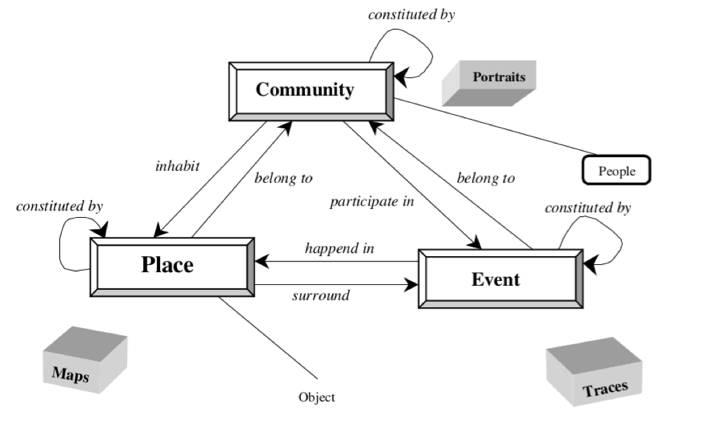
\includegraphics[scale=.5]{images/Figura2-1}
	\caption{\em Lógica de la 3-Ontology, extraído de Leiva-Lobos & Covarrubias (2002).}
	\label{fig:mt-im1}
\end{figure}

\begin{figure}
	\centering
	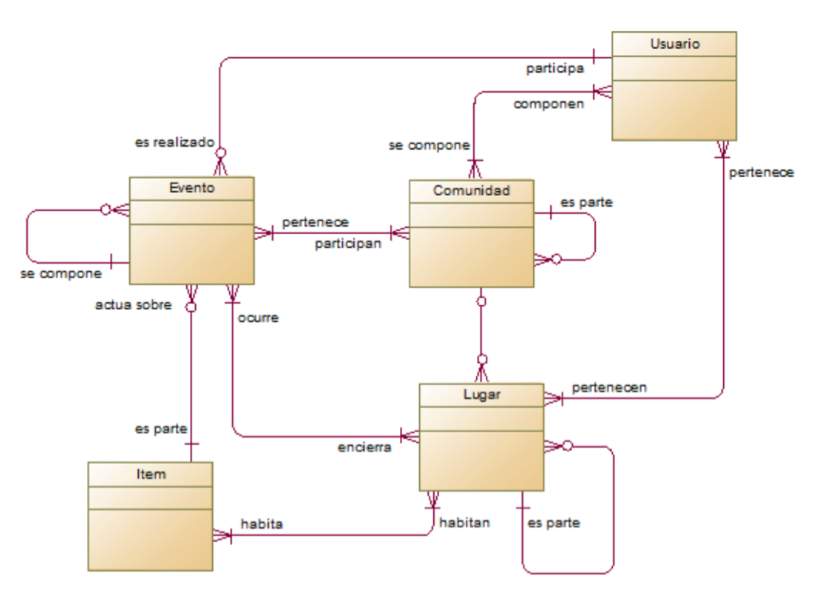
\includegraphics[scale=.5]{images/Figura2-2}
	\caption{\em Modelo conceptual de RBox, extraído de Vásquez (2013). }
	\label{fig:mt-im2}
\end{figure}

\section{Resumen}

En este capítulo se realizó una revisión de los fundamentos teóricos del trabajo de tesis. Para comenzar, se ha definido el concepto de red social. Luego, se presentó el concepto de análisis de redes sociales y los desafíos que supone para el área la inclusión de \textit{social media}. Posteriormente, se repasa el concepto de detección de comunidades y se explicitan distintas líneas de investigación. A continuación se trata el concepto de sistemas de recomendación de forma genérica y como han evolucionado a aquellos que consideran el contexto al momento de recomendar. Finalmente, se expone el concepto de la 3-Ontology, junto con los contenedores de sentido y se aborda una contribución de este trabajo de tesis a una implementación basada en este \textit{framework}.
